\documentclass[12pt]{beamer}
\usetheme{Madrid}
\usepackage{amsmath}
\usepackage{amssymb}%math symbols
\usepackage{bm}%fette Symbole(Vektoren)
\usepackage{nicefrac}
\usepackage{xcolor}
\usepackage{import}


\newcommand\Ccancel[2][black]{\renewcommand\CancelColor{\color{#1}}\xcancel{#2}}

\newcommand*{\HomePath}{} %Set Home Path

\graphicspath {{\HomePath Plots/}{Plots/}} %Set Plot Path
\subimport{}{commands.tex} %Import commands

\title{Rossby Waves}
\author{Philipp (all by himself)}
\institute{MPE}
\date{\today}

\begin{document}

 
\frame{\titlepage}
 
\begin{frame}
\frametitle{Vorticity Equation}
Rewrite  shallow water equations in terms of \textit{relative vorticity} $\zeta$
\vspace{0.5cm}
\begin{itemize}
\item take the curl $\nabla \times \left(...\right)$
\item $\pder{\zeta}{t}+\bm{u}\nabla(\zeta+f)=(\zeta+f)\nabla \bm{u}$
\end{itemize}
\vspace{0.5cm}
Inserting the mass conservation $\mder{h}{t}+h\nabla\bm{u}=0$, we can restate the equations as 
\vspace{0.5cm}
\begin{itemize}
\item $\mder{}{t}\left(\frac{\zeta+f}{h}\right)=0$
\end{itemize}
\vspace{0.5cm}
We found a conserved quantity! It is called \textbf{potential vorticity}. 
\end{frame}


\begin{frame}
\frametitle{Potential Vorticity}
What is potential vorticity $q=\frac{\zeta+f}{h}, \mder{}{t}q=0$?
\vspace{0.5cm}
\begin{itemize}
\item Continuum equivalent of \textit{angular momentum} conservation
\end{itemize}
\vspace{0.5cm}
In $f$-plane approximation, $f=f_0=$const. :
\vspace{0.2cm}
\begin{columns}
    \begin{column}{0.48\textwidth}
        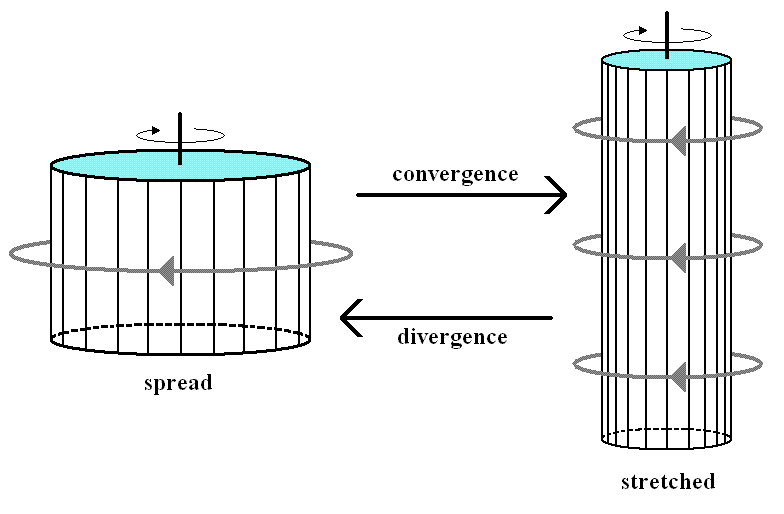
\includegraphics[width=\linewidth]{Potential_vorticity_conservation}
    \end{column}
    \begin{column}{0.48\textwidth}
       \begin{itemize}
	\item Change in $\zeta$ has to be compensated by change in hight $h$
	\end{itemize}
    \end{column}
\end{columns}
\end{frame}


\begin{frame}
\frametitle{Potential Vorticity}
In $\beta$-plane approximation $f=f_0+\beta y$ is not constant. \hfill $\color{blue}\boxed{q=\frac{\zeta+f}{h}}$\\
\vspace{0.5cm}
Fluid parcels can move north-/southward when changing vorticity $\zeta$.
\begin{columns}
    \begin{column}{0.55\textwidth}
        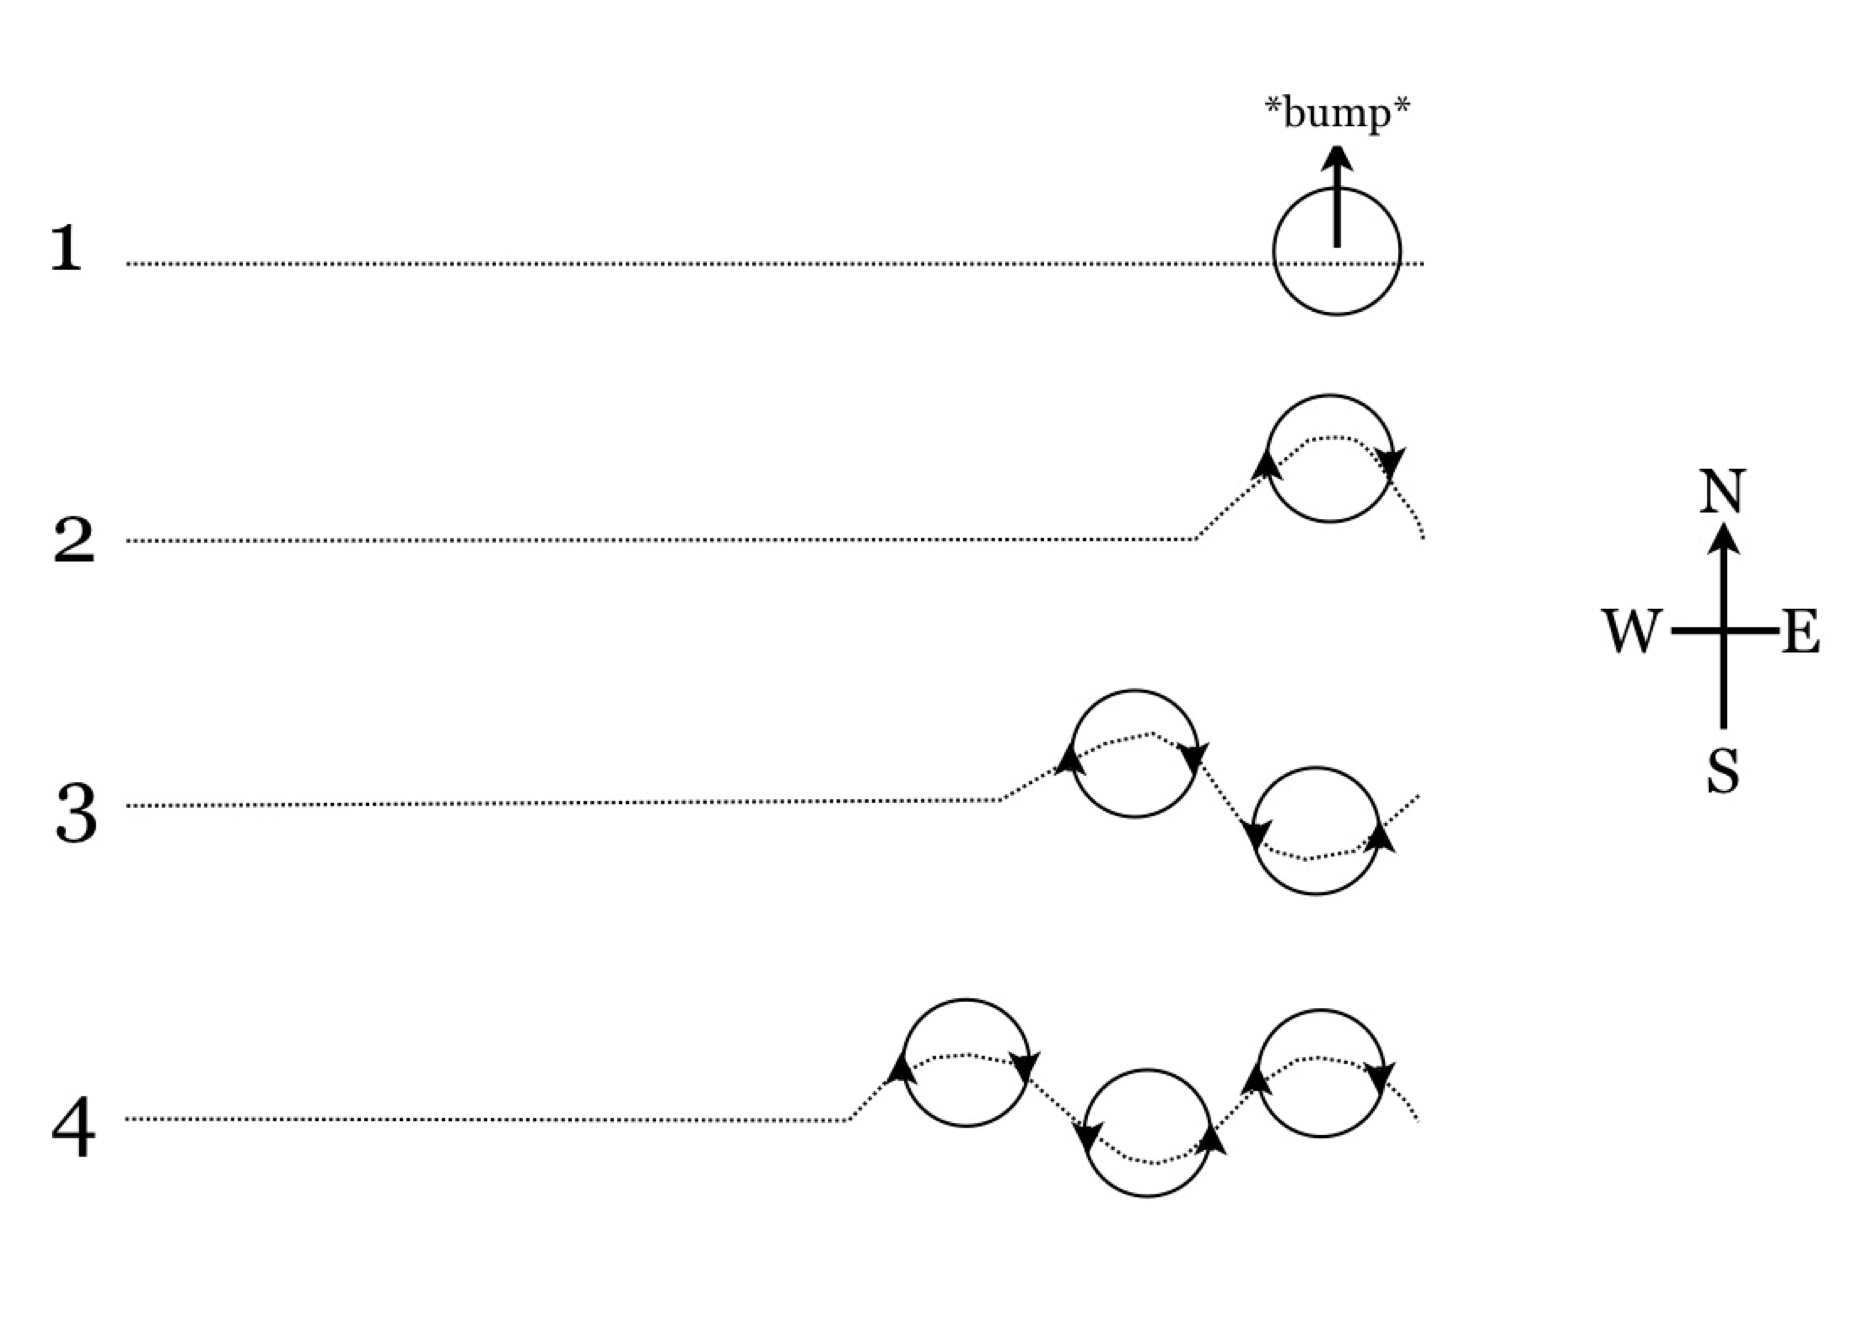
\includegraphics[width=\linewidth]{beta_plane}
    \end{column}
    \begin{column}{0.45\textwidth}
       \begin{itemize}
	\item Additionally induce movement on neighboured fluid particles
	\end{itemize}
    \end{column}
\end{columns}
\end{frame}
\end{document}